% !TeX root = ../main_problemset.tex
\documentclass[../main_problemset.tex]{subfiles} % Inherits definitions from parent .tex file.

% Per-problem variable definitions
\newcommand{\problemName}{H. Harta Kekayaan}
\newcommand{\problemTL}{4 s}
\newcommand{\problemML}{256 MB}

\begin{document}

\begin{center}
    \section*{\problemName}
    \addcontentsline{toc}{section}{\problemName} % for pdf indexing
    
    \begin{tabular}{rl}
    Batasan waktu : & \problemTL \\
    Batasan memori : & \problemML
    \end{tabular}
\end{center}

\subsection*{Deskripsi}
\addcontentsline{toc}{subsection}{Deskripsi} % for pdf indexing

Perusahaan Astik terdiri atas N karyawan, yang dinomori dari 1 hingga N. Setiap karyawan, kecuali karyawan 1, memiliki tepat seorang manajer, yang juga merupakan salah satu dari N karyawan tersebut. Manajer karyawan i adalah karyawan P[i]. Hubungan manajer-karyawan ini membentuk sebuah struktur \textit{tree} yang berakar pada karyawan 1.

Karyawan j adalah atasan dari karyawan i apabila j merupakan salah satu dari \{P[i], P[P[i]], P[P[P[i]]], ..., 1\}.

Pak Chanek adalah auditor keuangan untuk perusahaan Astik. Setiap karyawan melaporkan harta kekayaan masing-masing kepada Pak Chanek. Karyawan ke-i memiliki harta sebesar R[i].

Pak Chanek mendefinisikan fungsi audit(x, y) sebagai banyaknya karyawan z yang memenuhi seluruh syarat di bawah ini:

\begin{itemize}
	\item Karyawan z merupakan atasan karyawan x
	\item Karyawan z merupakan atasan karyawan y
	\item R[z] $ > $ R[x]
	\item R[z] $ > $ R[y]
\end{itemize}

Untuk laporan tahun ini, Pak Chanek harus menghitung jumlah dari audit(x, y) untuk seluruh 1 $ \le $ x $ < $ y $ \le $ N. Bantulah dia!

\subsection*{Format Masukan}
\addcontentsline{toc}{subsection}{Format Masukan} % for pdf indexing

Baris pertama berisi sebuah bilangan bulat T yang menyatakan banyaknya kasus uji. Baris-baris berikutnya berisi T kasus uji, yang masing-masing diberikan dalam format berikut ini:

\begin{lcverbatim}
N
P[2] P[3] .. P[N]
R[1] R[2] R[3] .. R[N]
\end{lcverbatim}

\subsection*{Format Keluaran}
\addcontentsline{toc}{subsection}{Format Keluaran} % for pdf indexing

Untuk setiap kasus uji, keluarkan sebuah baris berisi jumlah dari audit(x, y) untuk seluruh 1 $ \le $ x $ < $ y $ \le $ N.

\vspace{.4cm}

\begin{minipage}[t]{0.5\textwidth}
\subsection*{Contoh Masukan}
\addcontentsline{toc}{subsection}{Contoh Masukan} % for pdf indexing

\begin{lcverbatim}
1
6
1 1 1 4 4
3 6 1 4 2 1
\end{lcverbatim}
\end{minipage}
\begin{minipage}[t]{0.5\textwidth}
\subsection*{Contoh Keluaran}
\addcontentsline{toc}{subsection}{Contoh Keluaran} % for pdf indexing

\begin{lcverbatim}
4
\end{lcverbatim}
\end{minipage}

\pagebreak
\subsection*{Penjelasan}
\addcontentsline{toc}{subsection}{Penjelasan} % for pdf indexing

Berikut ini adalah ilustrasi \textit{tree} untuk contoh tersebut. Harta setiap karyawan tertera di sebelah kanan \textit{node}.

\begin{figure}[H]
	\centering
	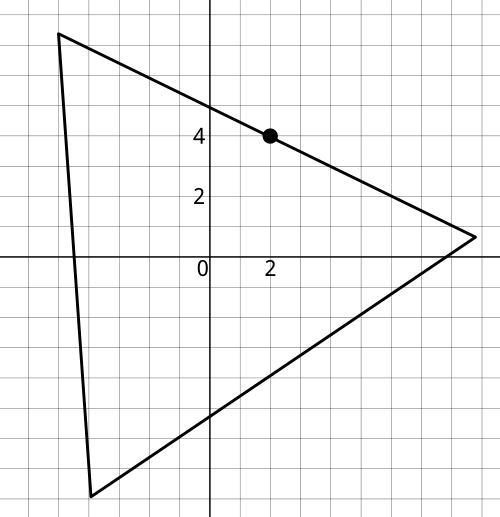
\includegraphics[width=160px]{richer/asset/1}
\end{figure}

\begin{itemize}
	\item audit(3, 5) = 1 (himpunan z yang memenuhi adalah \{1\})
	\item audit(3, 6) = 1 (himpunan z yang memenuhi adalah \{1\})
	\item audit(5, 6) = 2 (himpunan z yang memenuhi adalah \{1, 4\})
	\item audit(x, y) untuk pasangan (x, y) yang lain = 0
\end{itemize}

Maka, jumlahannya adalah 1 + 1 + 2 = 4.

\subsection*{Batasan}
\addcontentsline{toc}{subsection}{Batasan} % for pdf indexing

\begin{minipage}[t]{0.47\textwidth}

Batasan yang berlaku untuk versi mudah dan versi sulit:

\begin{itemize}
	\item 1 $ \leq $ T $ \leq $ 10
	\item 1 $ \leq $ P[i] $ < $ i, untuk i $ > $ 1
	\item 1 $ \le $ R[i] $ \le $ 100.000
\end{itemize}
\end{minipage}
\begin{minipage}[t]{0.06\textwidth}
	\hfill
\end{minipage}
\begin{minipage}[t]{0.47\textwidth}
Batasan khusus versi mudah:
\begin{itemize}
	\item 2 $ \le $ N $ \le $ 2.000
\end{itemize}

\vspace{.2cm}

Batasan khusus versi sulit:
\begin{itemize}
	\item 2 $ \le $ N $ \le $ 100.000
\end{itemize}
\end{minipage}

\end{document}
